\documentclass[aps,prl,superscriptaddress,12pt]{revtex4-1}
	\usepackage{graphicx}  % needed for figures
	\usepackage{fancyhdr} % needed for team number and page number
	\usepackage{amsmath}
	\usepackage{comment}
	% configure desired header format
	\pagestyle{fancy}
	\fancyhf{}
	\lhead{ Team \#  }
	\rhead{ Page \thepage\text{ }of \pageref{LastPage} }

\begin{document}

	\title{Macroscopic and Microscopic Assessment of Traffic Rules }
	%\author{Abigail Chua}
	%	\affiliation{Denison University, Granville, OH, 43023, USA}
	%\author{Yubo Yang}
	%	\affiliation{Denison University, Granville, OH, 43023, USA}
	%\author{Yifu Zhao}
	%	\affiliation{Denison University, Granville, OH, 43023, USA}
		
	\begin{abstract}
		Summary goes here
	\end{abstract}
	
\maketitle

	\section{Interpretation of the Problem}

	\section{Introduction}
		Our writing style should follow guidelines such as \cite{science_writing}.

	\section{Model}
	
	\begin{table}
	\begin{tabular}{|c|c|c|} \hline
	quantity & variable & unit \\ \hline
	position on the freeway & x & m/s \\ \hline
	traffic density on lane 1 & $\rho_1(x,t)$ & cars/m \\ \hline
	traffic density on lane 2 & $\rho_2(x,t)$ & cars/m \\ \hline
	average velocity on lane 1 & $v_1(x,t)$ & m/s \\ \hline
	average velocity on lane 2 & $v_2(x,t)$ & m/s \\ \hline
	\end{tabular}
	\caption{ variables used in the macroscopic model \label{tab:variables} }
	\end{table}	
	
	To simplify the model, we consider a stretch of straight two-lane freeway with no on/off ramp. To assess the performance of the given traffic rule, we would like to analyze its capacity for traffic flow under both heavy and light traffic conditions. Traffic flow rate is best captured in a macroscopic model with variables shown in Table \ref{tab:variables}. The total amount of traffic flow will then be determined by 
	
	\begin{align}
	& Q(x,t) = \rho_1(x,t)\cdot v_1(x,t)+\rho_2(x,t)\cdot v_2(x,t) &
	\end{align}
	
	We further assume that at equilibrium, there is some velocity-density relation. Given this velocity-density relation, the flow at any given junction of the freeway at a given time is completely determined by the local traffic densities $\rho_1$ and $\rho_2$. 
Kerner elt. al. proposed the following relationship in 2002. 
	\begin{align}
	& v_e = v_o\left( (\frac{1+e^{\rho/\rho_m-0.25}}{0.06})^{-1} - 3.76\times10^{-6} \right) & \label{eq:Kerner}
	\end{align}
	It captures the key 
	\begin{figure}
	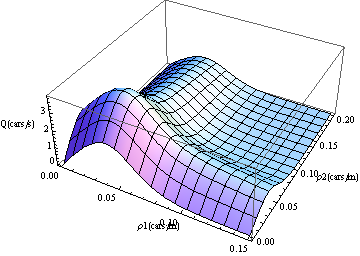
\includegraphics[scale=1]{plot/Q_p1_p2}
	\caption{equilibrium traffic flow as a function of traffic densities using Kerner's velocity-density relation\label{fig:Q_p1_p2}}
	\end{figure}
	
	
	To derive such a relation, we consider all cars to have uniform length $l(m)$, travel with uniform velocity $v_e(\rho)$ and maintain uniform bumper-to-bumper distance $d(m)$ from their neighbors. At this equilibrium, each car will take up a total space of $d+l$ on one lane of the freeway. Therefore, the density of cars
	\begin{align}
	& \rho = \frac{1}{d+l} & \label{eq:follow}
	\end{align}
	Incorporating the two-second rule enforced by the New York Sate Department of Motor Vehicles \cite{science_writing}, $d=2v_e(\rho)$, equation (\ref{eq:follow}) can be solved to obtain and expression for $v_e(\rho)$
	\begin{align}
	& v_e(\rho) =  .5(\frac{1}{\rho}-l)& 
	\end{align}
	
	\pagebreak

	\section{Result}

	\section{Discussion}
	
\bibliographystyle{unsrt}
\bibliography{ref/ref}
\end{document}